% 使用自定义文档类
\documentclass{../pkslide}




% =============================================================================
% 以下是导言区



% ===================================================================
% 调用宏包


% \usepackage{relsize}


\usepackage{tikz}


\usepackage{minted}


\usepackage{changepage}


\usepackage{graphbox}


% 目前最新的画表格宏包
\usepackage{tabularray}



% ===================================================================
% 自定义一些命令


% C++ 符号宏,依赖 hyperref 和 relsize
% 来自 GitHub 上的仓库 tcbrindle/wg21papertemplate 中的 ./common.tex 文件
\newcommand{\Cpp}{\texorpdfstring{C\kern-0.05em\protect\raisebox{.35ex}{\textsmaller[2]{+\kern-0.05em+}}}{C++}}


% 用于数学公式中的自定义命令
\newcommand{\nequiv}{\not\equiv} % 不同余
\newcommand{\lcm}{\operatorname{lcm}} % 最小公倍数
\newcommand{\lpd}{\operatorname{lpd}} % 最小素因数


\SetTblrInner{rowsep = 0pt} % tabularry : match the original array
\SetTblrInner{colsep = 5pt} % tabularry : match the original array


\newcommand{\textboldcolor}[2]{\textcolor{#1}{\bfseries{}\boldmath{}#2\unboldmath{}}}
\newcommand{\fdf}[1]{\textboldcolor{red}{#1}}



% ===================================================================
% 不影响显示形式的,需要在导言区引入的信息


% 标题、作者、学校/机构与日期信息,用于标题页显示和页脚显示:页脚将会显示短形式
\title[算法竞赛中的数论(一)]{算法竞赛中的数论}
\subtitle{\texorpdfstring{\textsuperscript{1.}}{1. }基础知识、简单素数筛法、与解线性 Diophantus 方程}
\firstauthor{%
  陈亮舟%
  %\inst{1}%
}[PinkRabbit]
\firstinstitute{%
  %\inst{1}%
  福建师范大学附属中学%
}[The Affiliated High School of Fujian Normal University]{AHSFNU}
\originalfinaldate[2022 年 1 月 26 日]{\today}



% 以上是导言区
% =============================================================================

\begin{document}

\section{基础知识}
\subsection{小学数学知识}
\subsubsection{小学课内数学}

% \iffalse %%%%%%%%%%%%%%%%%%%%%%%%%%%%%%%%%%%%%%%%%%%%%%%%%%%%%%

\begin{frame}
  \frametitle{整除性}
  
  \begin{definition}[整除、因数与倍数]
    对于整数 $a, b$,且 $a \ne 0$,如果 \textcolor{blue}{$\frac{b}{a}$ 也是整数},则称 \fdf{$b$ 被 $a$ 整除},或称 \fdf{$a$ 整除 $b$},记作 \fdf{$a \mid b$},否则称 $a$ 不整除 $b$,记作 \fdf{$a \nmid b$}。
   
    若 $a$ 整除 $b$,也称 $b$ 是 $a$ 的\fdf{倍数},$a$ 是 $b$ 的\fdf{因数(约数)}。
    
    \emptyline
    
    \visible<2>{
      同时,我们\alert{约定} $0$ 整除 $0$,但不整除其他任何整数。
      
      即 $0 \mid 0$,但是对于所有 $n \ne 0$ 均有 $0 \nmid n$。
    }
  \end{definition}
\end{frame}

\begin{frame}
  \frametitle{整除性 -- 例子}
  
  \only<1-3>{
    \begin{examples}[整除性]
      \begin{itemize}
        \item<2-> $\phantom{-}2$ \hspace{1em}整除 $\phantom{-}6$,因为 $\frac{6}{2} = 3$ 是整数。
        \item<2-> $-6$ \hspace{1em}整除 $\phantom{-}6$,因为 $\frac{6}{-6} = -1$ 是整数。
        \item<2-> $\phantom{-}5$ \hspace{1em}整除 $\phantom{-}0$,因为 $\frac{0}{5} = 0$ 是整数。
        \item<2-> $-4$ 不整除 $-6$,因为 $\frac{-6}{-4} = 1.5$ 不是整数。
        \item<3 > $\phantom{-}0$ \hspace{1em}整除 $\phantom{-}0$,因为我们约定如此。
        \item<3 > $\phantom{-}0$ 不整除 $-7$,因为我们约定如此。
      \end{itemize}
    \end{examples}
  }
  
  \only<4-6>{
    \begin{examples}[因数与倍数]
      \begin{itemize}
        \item<5-> 所以 $\phantom{-}6$ \hspace{1em}是 $\phantom{-}2$ 的倍数,$\phantom{-}2$ \hspace{1em}是 $\phantom{-}6$ 的因数。
        \item<5-> \-\hspace{2em} $\phantom{-}6$ \hspace{1em}是 $-6$ 的倍数,$-6$ \hspace{1em}是 $\phantom{-}6$ 的因数。
        \item<5-> \-\hspace{2em} $\phantom{-}0$ \hspace{1em}是 $\phantom{-}5$ 的倍数,$\phantom{-}5$ \hspace{1em}是 $\phantom{-}0$ 的因数。
        \item<5-> \-\hspace{2em} $-6$ 不是 $-4$ 的倍数,$-4$ 不是 $-6$ 的因数。
        \item<6 > \-\hspace{2em} $\phantom{-}0$ \hspace{1em}是 $\phantom{-}0$ 的倍数,$\phantom{-}0$ \hspace{1em}是 $\phantom{-}0$ 的因数。
        \item<6 > \-\hspace{2em} $-7$ 不是 $\phantom{-}0$ 的倍数,$\phantom{-}0$ 不是 $-7$ 的因数。
      \end{itemize}
    \end{examples}
  }
\end{frame}

\begin{frame}
  \frametitle{整除性 -- 基本性质}
  
  关于整除的一些基本性质:
  
  \begin{itemize}
    \setlength{\itemsep}{2pt}
    \item<2-> 对于任意整数 $a$,均有 $a \mid a$(自反性)以及 $a \mid (-a)$。
    \item<2-> 如果 $a \mid b$ 且 $b \mid c$,那么 $a \mid c$。(传递性)
    \item<3-> 如果 $a \mid b$ 且 $b \ne 0$,那么 $|a| \le |b|$。
    \item<3-> 如果 $a \mid b$ 且 $b \mid a$,那么 $a = \pm b$。
    \item<4-> 如果 $a \mid b$ 且 $k$ 为整数,那么 $a \mid (k \cdot b)$ 且 $(k \cdot a) \mid (k \cdot b)$。
    \item<4-> 如果 $d \mid a$ 且 $d \mid b$,那么 $d \mid (a \pm b)$。
    \item<5-> 一般地,如果有 $n$ 个整数 $a_1, a_2, \ldots, a_n$,对于 $i = 1 \sim n$ 均有 $d \mid a_i$,且另给 $n$ 个整数 $k_1, k_2, \ldots, k_n$,则有%
      %
      \begin{center}
        $\displaystyle d \mid (k_1 a_1 + k_2 a_2 + \cdots + k_n a_n)$。
      \end{center}%
      %
      \visible<6>{其中 $k_1 a_1 + k_2 a_2 + \cdots + k_n a_n$ 被称作 $a_{1 \sim n}$ 的{\color{red} \textbf{整系数线性组合}}。}
  \end{itemize}
\end{frame}

\begin{frame}
  \frametitle{整除性 -- 简单规律}
  
  关于整除的一些简单规律:
  
  \begin{itemize}
    \item<2-> $1$ 和 $-1$ 整除所有整数。\\
      $1$ 和 $-1$ 是所有整数的因数,所有整数是 $1$ 和 $-1$ 的倍数。
    \item<3-> 所有整数整除 $0$。\\
      $0$ 是所有整数的倍数,所有整数是 $0$ 的因数。
    \item<4-> 对于正整数 $a$,$a$ 是 $a$ 的最大因数,也是 $a$ 的最小正倍数。\\
      并且,$-a$ 是 $a$ 的最小因数,也是 $a$ 的最大负倍数。
  \end{itemize}
  
  \visible<5>{
    一般地,对于任意整数 $a$,一定有 $1, -1, a, -a$ 是 $a$ 的因数,\\
    \-\hspace{10em}\hphantom{ $a$}也一定有 $\phantom{0, -{}}0, a, -a$ 是 $a$ 的倍数。
    
    对于非 $0$ 整数 $a$,称 $1, -1, a, -a$ 为 $a$ 的\fdf{平凡因数}。
  }
\end{frame}

\begin{frame}
  \frametitle{有余数的除法}
  
  \begin{definition}[有余数的除法]
    对于整数 $a$ 和正整数 $m$,存在且仅存在一对整数 $\langle q, r \rangle$ 满足%
    %
    \begin{center}
      $a = q \cdot m + r$ 且 $0 \le r < m$,
    \end{center}%
    %
    称 $a$ 除以 $m$ 的\hspace{.5em}\fdf{商}\hspace{.5em}为 $q$,\\
    \-\hspace{1em} $a$ 除以 $m$ 的\fdf{余数}为 $r$。
    
    记作 $a \div m = q \cdots \cdots r$。
  \end{definition}
\end{frame}

\begin{frame}
  \frametitle{有余数的除法 -- 例子}
  
  \begin{examples}[有余数的除法]
    \begin{itemize}
      \item $8$ 除以 $3$ 的商为 $2$,余数为 $2$。\\
        因为 $2 \times 3 + 2 = 8$,且 $0 \le 2 < 3$。
      \item $-9$ 除以 $5$ 的商为 $-2$,余数为 $1$。\\
        因为 $(-2) \times 5 + 1 = -9$,且 $0 \le 1 < 5$。
      \item $-12$ 除以 $4$ 的商为 $-3$,余数为 $0$。\\
        因为 $(-3) \times 4 + 0 = -12$,且 $0 \le 0 < 4$。
      \item ${10}^6$ 除以 $7$ 的商为 $142857$,余数为 $1$。\\
        因为 $142857 \times 7 + 1 = {10}^6$,且 $0 \le 1 < 7$。
    \end{itemize}
  \end{examples}
  
  \visible<2>{注意到,如果 $a$ 除以 $m$ 的余数为 $0$,则 $m \mid a$,否则 $m \nmid a$。}
\end{frame}

\begin{frame}
  \frametitle{\Cpp{} 中的除法和求余运算符}
  
  \only<1>{
    在 \Cpp{} 中,提供了除法运算符“\texttt{/}”和求余运算符“\texttt{\%}”以支持 \Cpp{} 程序进行相关计算。它们的形式为:
    
    \begin{itemize}
      \item “\texttt{\textcolor{darkgray}{左操作数} / \textcolor{darkgray}{右操作数}}”,
      \item “\texttt{\textcolor{darkgray}{左操作数} \% \textcolor{darkgray}{右操作数}}”。
    \end{itemize}
    
    这里我们针对两操作数均拥有整数类型或无作用域枚举类型的情况进行说明。假设两操作数已进行过整型提升和整型转换,并产生为 \texttt{int} 或 \texttt{long long} 及其无符号(\texttt{unsigned})版本之一的公共类型。
  }
  
  \only<2-4>{
    从 \Cpp{}11 标准开始,规定了除法运算符的舍入方向:运算结果为第一操作数除以第二操作数的数值结果\alert{向零舍入}得到的整数。
    
    这意味着,如果数值结果 $> 0$,则运算结果 $\le$ 数值结果,\\
    \-\hspace{5em}如果数值结果 $< 0$,则运算结果 $\ge$ 数值结果,\\
    \-\hspace{5em}如果数值结果 $= 0$,则运算结果 $=$ 数值结果 $= 0$。
    
    \visible<3->{
      \emptyline
      
      注意,\Cpp{} 中除法和求余运算符的第二操作数均可以为负数,这与前文中“有余数的除法”不同。
    }
    
    \visible<4>{
      \emptyline
      
      特别地,如果第二操作数为 $0$,则行为未定义(UB)。典型的编译器实现可能导致运行时错误(RE)。
      
      若运算结果不能以结果类型表示,则行为未定义。
    }
  }
\end{frame}

\begin{frame}
  \frametitle{\Cpp{} 中的除法和求余运算符 -- 除法运算符例子}
  
  \begin{examples}[除法运算符]
    \begin{itemize}
      \item<2-> \texttt{ 5 / \ 3} 的结果为 \texttt{ 1}。
      \item<2-> \texttt{ 5 / -3} 的结果为 \texttt{-1}。
      \item<2-> \texttt{-5 / \ 3} 的结果为 \texttt{-1}。
      \item<2-> \texttt{-5 / -3} 的结果为 \texttt{ 1}。
      \item<3-> \texttt{-7 / \ 0} 是未定义行为。
      \item<3-> \texttt{ 0 / \ 0} 是未定义行为。
      \item<4-> \texttt{(int)(-2147483648LL) / -1} 是未定义行为(补码系统上)。
    \end{itemize}
  \end{examples}
\end{frame}

\begin{frame}
  \frametitle{\Cpp{} 中的除法和求余运算符 -- 求余运算符}
  
  对于求余运算符,\Cpp{} 保证了:若 $a \mathbin{\texttt{\%}} m = r$ 以及 $a \mathbin{\texttt{/}} m = q$,则一定有 $a = q \mathbin{\texttt{*}} m \mathbin{\texttt{+}} r$。(前提是 $a \mathbin{\texttt{/}} m$ 时不会触发未定义行为)
  
  \emptyline
  
  \visible<2>{所以,对于非负数 $a$ 和正数 $m$,\Cpp{} 产生的商和余数与前文“有余数的除法”中定义的相同。}
\end{frame}

\begin{frame}
  \frametitle{\Cpp{} 中的除法和求余运算符 -- 求余运算符例子}
  
  \begin{examples}[求余运算符]
    \begin{itemize}
      \item<2-> \texttt{ 5 \% \ 3} 的结果为 \texttt{ 2}。
      \item<2-> \texttt{ 5 \% -3} 的结果为 \texttt{ 2}。
      \item<2-> \texttt{-5 \% \ 3} 的结果为 \texttt{-2}。
      \item<2-> \texttt{-5 \% -3} 的结果为 \texttt{-2}。
      \item<3-> \texttt{-7 \% \ 0} 是未定义行为。
      \item<3-> \texttt{ 0 \% \ 0} 是未定义行为。
      \item<4-> \texttt{(int)(-2147483648LL) \% -1} 是未定义行为(补码系统上)。
    \end{itemize}
  \end{examples}
\end{frame}

\begin{frame}
  \frametitle{\Cpp{} 中的除法和求余运算符 -- 正负性提示}
  
  假设 $a \mathbin{\texttt{/}} m = q$ 和 $a \mathbin{\texttt{\%}} m = r$。
  
  则有 $q$ 的正负性与 $a \cdot m$ 的正负性相同,\\
  \-\hspace{2em} $r$ 的正负性与 $a$ 的正负性相同。
  
  \emptyline
  
  \visible<2>{在操作数可能为负数或 $0$ 时,需要特别注意。}
\end{frame}

\begin{frame}
  \frametitle{素数与合数}
  
  \only<1-3>{
    \begin{definition}[素数]
      恰好有 $2$ 个正因数的正整数称为\fdf{素数(质数,prime number)}。
      
      即,唯二的两个正因数为 $1$ 和它本身。
    \end{definition}
    
    \visible<2->{
      \begin{examples}[素数]
        \begin{itemize}
          \item $7$ 是素数,因为 $7$ 恰好有 $2$ 个正因数 $1, 7$。
          \item $51$ 不是素数,因为 $51$ 有 $4$ 个正因数 $1, 3, 17, 51$。
          \item $1$ 不是素数,因为 $1$ 只有 $1$ 个正因数 $1$。
          \item $-7$ 不是素数,因为 $-7$ 不是正整数。
        \end{itemize}
      \end{examples}
    }
    
    \visible<3>{
      若无特殊说明,下文中的字母 $p$ 均表示素数,$\mathbb P$ 为素数集。
    }
  }
  
  \only<4-6>{
    这里列举一下前几个素数:
    
    \begin{center}
      $\mathbb P = \{ 2, 3, 5, 7, 11, 13, 17, 19, 23, 29, 31, 37, 41, 43, 47, 53, \ldots \}$。
    \end{center}
    
    \visible<5->{
      \begin{definition}[合数]
        有多于 $2$ 个正因数的正整数称为\fdf{合数}。
        
        即,除了 $1$ 和它本身还有别的正因数。
        
        注意 $1$ 既不是素数也不是合数。
      \end{definition}
    }
    
    \visible<6->{
      这里列举一下前几个合数:
      
      \begin{center}
        $\mathbb{Z}_{\ge 2} \setminus \mathbb{P} = \{ 4, 6, 8, 9, 10, 12, 14, 15, 16, 18, 20, 21, 22, 24, 25, 26, \ldots \}$。
      \end{center}
    }
  }
\end{frame}

% \fi %%%%%%%%%%%%%%%%%%%%%%%%%%%%%%%%%%%%%%%%%%%%%%%%%%%%%%%%%%%

\subsubsection{小学奥数}

% \iffalse %%%%%%%%%%%%%%%%%%%%%%%%%%%%%%%%%%%%%%%%%%%%%%%%%%%%%%

\begin{frame}
  \frametitle{同余}
  
  \begin{definition}[同余和模]
    对于正整数 $m$ 和整数 $a, b$,如果 $a, b$ 的差被 $m$ 整除,即 $m \mid (a - b)$,则称 \fdf{$a$ 同余于 $b$ 模 $m$}。
    
    换句话说,$a$ 除以 $m$ 的余数等于 $b$ 除以 $m$ 的余数。
    
    记作 \fdf{$a \equiv b \pmod{m}$},并称 $m$ 为\fdf{模数}。
    
    如果 $m \nmid (a - b)$,则称 $a$ 不同余于 $b$ 模 $m$,记作 $a \nequiv b \pmod{m}$。
    
    \visible<2->{
      \emptyline
      
      固定模 $m$ 下的同余关系是一种等价关系,即如果 $a \equiv b$ 且 $b \equiv c$,则 $a \equiv c$。还可以记作 $a \equiv b \equiv c \pmod{m}$。
    }
    
    \visible<3->{
      \emptyline
      
      若 $a$ 除以 $m$ 的余数为 $r$,也可以称 \fdf{$a$ 对 $m$ 的模为 $r$},\\
      或称 \fdf{$a$ 模 $m$ 等于 $r$}。记作 \fdf{$a \bmod m = r$}。
    }
  \end{definition}
\end{frame}

\begin{frame}
  \frametitle{同余 -- 例子}
  
  \begin{examples}[同余]
    \begin{itemize}
      \item<2-> $-2 \equiv 4 \pmod{3}$ 并且 $6 \nequiv 7 \pmod{3}$。
      \item<3-> 如果 $\mathcal{A} \equiv \mathcal{B} \pmod{m}$,且 $\mathcal{C} \equiv \mathcal{D} \pmod{m}$,则\\
        \-\hspace{2em} $(\mathcal{A}) \pm (\mathcal{C}) \equiv (\mathcal{B}) \pm (\mathcal{D}) \pmod{m}$,以及\\
        \-\hspace{2em} $(\mathcal{A}) \cdot (\mathcal{C}) \equiv (\mathcal{B}) \cdot (\mathcal{D}) \pmod{m}$。\\
        其中 $\mathcal{A}, \mathcal{B}, \mathcal{C}, \mathcal{D}$ 为任意取值为整数的数学表达式。
      \item<4-> 如果 $\mathcal{A} \equiv \mathcal{B} \pmod{m}$,则对于任意正整数 $k$,有\\
        \-\hspace{2em} $k \cdot (\mathcal{A}) \equiv k \cdot (\mathcal{B}) \pmod{k \cdot m}$。
      \item<5-> 如果 $\mathcal{A} \equiv \mathcal{B} \pmod{m}$,且 $k \mid \mathcal{A}$、$k \mid \mathcal{B}$、$k \mid m$,则\\
        \-\hspace{2em} $\frac{\mathcal{A}}{k} \equiv \frac{\mathcal{B}}{k} \pmod{\frac{m}{k}}$。
    \end{itemize}
  \end{examples}
\end{frame}

\begin{frame}
  \frametitle{最大公因数与最小公倍数 -- 公因数}
  
  \begin{definition}[公因数与最大公因数]
    对于整数 $a, b$,若存在整数 $d$ 使得 $d \mid a$ 且 $d \mid b$,则称 $d$ 是 $a, b$ 的一个\fdf{公因数}。$a, b$ 的公因数中的最大值称为 $a, b$ 的\fdf{最大公因数(greatest common divisor)},记作 \fdf{$\gcd(a, b)$}。
    
    特别地,约定 $0$ 与 $0$ 的最大公因数为 $\gcd(0, 0) = 0$。
    
    \visible<2->{
      \emptyline
      
      对于 $n$ 个整数 $a_1, a_2, \ldots, a_n$,若存在整数 $d$ 使得对于 $i = 1 \sim n$ 均有 $d \mid a_i$,则称 $d$ 是 $a_1, a_2, \ldots, a_n$ 的一个公因数。\\
      $a_1, a_2, \ldots, a_n$ 的公因数中的最大值称为 $a_1, a_2, \ldots, a_n$ 的最大公因数,记作 $\gcd(a_1, a_2, \ldots, a_n)$。
      
      特别地,若 $a_i$ 全部为 $0$,约定最大公因数为 $\gcd(0, 0, \ldots, 0) = 0$。
    }
  \end{definition}
\end{frame}

\begin{frame}
  \frametitle{最大公因数与最小公倍数 -- 公因数例子}
  
  \begin{examples}[公因数与最大公因数]
    \begin{itemize}
      \item<2-> $60$ 与 $96$ 的公因数有 $\{ \pm 1, \pm 2, \pm 3, \pm 4, \pm 6, \pm 12 \}$。
      \item<2-> $-60$ 与 $-96$ 的最大公因数为 $\gcd(-60, -96) = 12$。
      \item<3-> $0$ 与 $0$ 的最大公因数为 $\gcd(0, 0) = 0$。
      \item<3-> $6, 10, 15$ 的最大公因数为 $\gcd(6, 10, 15) = 1$。
    \end{itemize}
  \end{examples}
  
  \visible<4>{
    \begin{definition}[互素]
      如果 $\gcd(a, b) = 1$,那么称 \fdf{$a$ 与 $b$ 互素}。记作 \fdf{$a \perp b$}。
      
      如果 $\gcd(a_1, a_2, \ldots, a_n) = 1$,那么称 $a_1, a_2, \ldots, a_n$ 互素,但未必两两互素。
    \end{definition}
  }
\end{frame}

\begin{frame}
  \frametitle{最大公因数与最小公倍数 -- 公倍数}
  
  \begin{definition}[公倍数与最小公倍数]
    对于整数 $a, b$,若存在整数 $m$ 使得 $a \mid m$ 且 $b \mid m$,则称 $m$ 是 $a, b$ 的一个\fdf{公倍数}。$a, b$ 的公倍数中的最小正值称为 $a, b$ 的\fdf{最小公倍数(least common multiple)},记作 \fdf{${\lcm(a, b)}$}。
    
    特别地,约定任何整数 $a$ 与 $0$ 的最小公倍数为 $0$。
    
    \emptyline
    
    \visible<2>{
      对于 $n$ 个整数 $a_1, a_2, \ldots, a_n$,若存在整数 $m$ 使得对于 $i = 1 \sim n$ 均有 $a_i \mid m$,则称 $m$ 是 $a_1, a_2, \ldots, a_n$ 的一个公倍数。\\
      $a_1, a_2, \ldots, a_n$ 的公倍数中的最小正值称为 $a_1, a_2, \ldots, a_n$ 的最小公倍数,记作 $\lcm(a_1, a_2, \ldots, a_n)$。
      
      特别地,若 $a_i$ 中至少有一个为 $0$,约定最小公倍数为 $0$。
    }
  \end{definition}
\end{frame}

\begin{frame}
  \frametitle{最大公因数与最小公倍数 -- 公倍数例子}
  
  \begin{examples}[公倍数与最小公倍数]
    \begin{itemize}
      \item<2-> $60$ 与 $96$ 的公倍数有 $\{ \ldots, -960, -480, 0, 480, 960, \ldots \}$。
      \item<2-> $-60$ 与 $-96$ 的最小公倍数为 $\lcm(-60, -96) = 480$。
      \item<3-> $-60$ 与 $0$ 的最小公倍数为 $\lcm(-60, 0) = 0$。
      \item<3-> $6, 10, 15$ 的最小公倍数为 $\lcm(6, 10, 15) = 30$。
      \item<4> 如果 $a \perp b$,那么 $\lcm(a, b) = |a| \cdot |b|$。\\
        否则,也有 $\lcm(a, b) = \frac{|a| \cdot |b|}{\gcd(a, b)}$($a, b$ 不能同时为 $0$)。
    \end{itemize}
  \end{examples}
\end{frame}

% \fi %%%%%%%%%%%%%%%%%%%%%%%%%%%%%%%%%%%%%%%%%%%%%%%%%%%%%%%%%%%

\subsection{算术基本定理}
\subsubsection{算术基本定理}

% \iffalse %%%%%%%%%%%%%%%%%%%%%%%%%%%%%%%%%%%%%%%%%%%%%%%%%%%%%%

\begin{frame}
  \frametitle{算术基本定理}
  
  \begin{theorem}[算术基本定理(fundamental theorem of arithmetic)]
    对于任意正整数 $n$,$n$ 可以表示成有限个素数的乘积(允许重复)。\\
    即 $n = p_1^{\alpha_1} p_2^{\alpha_2} \cdots p_k^{\alpha_k}$,其中 $p_1 < p_2 < \cdots < p_k$ 为递增素数,$\alpha_1, \alpha_2, \ldots, \alpha_k$ 为正整数。并且这种表示方法是唯一的,称为 $n$ 的\fdf{标准分解式}。
    
    当 $n = 1$ 时,可视作 $k = 0$,即 $1$ 可以表示成 $0$ 个素数的乘积(我们约定 $0$ 个数的乘积为 $1$)。
  \end{theorem}
  
  \visible<2>{
    \begin{examples}[标准分解式]
      \begin{mymulticols}[l][l]{2}
        \begin{itemize}
          \item $10725 = 3^1 \cdot 5^2 \cdot {11}^1 \cdot {13}^1$
          \item $998244352 = 2^{23} \cdot {7}^1 \cdot {17}^1$
        \end{itemize}
      \end{mymulticols}
    \end{examples}
  }
\end{frame}

\begin{frame}
  \frametitle{算术基本定理 -- 证明(存在性)}
  
  \begin{proof}[算术基本定理 -- 存在性]
    如果 $n = 1$ 或 $n$ 是素数,则显然存在表示方法。
    
    否则 $n$ 是合数,存在非 $1$ 或其本身的正因数 $a$,令 $b = \frac{n}{a}$,则 $a, b < n$,可以递归地求出 $a, b$ 的表示方法:$a = p_1^{\alpha_1} p_2^{\alpha_2} \cdots p_k^{\alpha_k}$ 和 $b = q_1^{\beta_1} q_2^{\beta_2} \cdots q_l^{\beta_l}$,将两个表示方法进行归并即可得到 $n$ 的表示方法。
  \end{proof}
\end{frame}

\begin{frame}
  \frametitle{算术基本定理 -- 证明(唯一性)}
  
  \only<1-5>{
    \begin{proof}[算术基本定理 -- 唯一性]
      \renewcommand{\qedsymbol}{\visible<5>{(续)}}
      
      假设存在正整数拥有多于一种表示方法,令其中最小的数为 $n$。\\
      显然,满足条件的 $n$ 必须为合数。
      
      \visible<2->{
        设 $n$ 的两种表示方法为 $p_1^{\alpha_1} p_2^{\alpha_2} \cdots p_k^{\alpha_k}$ 和 $q_1^{\beta_1} q_2^{\beta_2} \cdots q_l^{\beta_l}$。
      }
      
      \visible<3->{
        \emptyline
        
        令 $P = p_1^{\alpha_1 - 1} p_2^{\alpha_2} \cdots p_k^{\alpha_k}$ 以及 $Q = q_1^{\beta_1 - 1} q_2^{\beta_2} \cdots q_l^{\beta_l}$。
      
        那么 $p_1 P = q_1 Q = n$,且 $2 \le P, Q < n$。
      }
      
      \begin{itemize}
        \item<4-> 如果 $p_1 = q_1$,那么 $P = Q < n$ 拥有两种表示方法,与 $n$ 的最小性矛盾。
        \item<5> 否则 $p_1 \ne q_1$,不失一般性,设 $p_1 < q_1$,则 $Q < P < n$。
      \end{itemize}
    \end{proof}
  }
  
  \only<6-11>{
    \begin{proof}[算术基本定理 -- 唯一性(续)]
      \renewcommand{\qedsymbol}{\visible<11>{\leavevmode \hbox {\usebeamertemplate *{qed symbol}}}}
      
      \begin{itemize}
        \item 否则 $p_1 \ne q_1$,不失一般性,设 $p_1 < q_1$,则 $Q < P < n$。
          
          \visible<7->{令 $s = p_1 \cdot (P - Q)$,则 $2 \le s < n$,然而同时 $s = (q_1 - p_1) \cdot Q$。}
          
          \visible<8->{由 $s < n$ 可知 $s$ 的表示方法唯一。注意到 $p_1 \cdot (P - Q)$ 中包含 $p_1$,这说明 $q_1 - p_1$ 或 $Q$ 中必然包含 $p_1$。}
          
          \visible<9->{然而 $p_1 \mid (q_1 - p_1) \iff p_1 \mid q_1$ 是不可能的,因为 $q_1$ 是素数。}
          
          \visible<10->{并且 $p_1 \mid Q$ 也是不可能的,因为由 $Q < n$ 可知 $Q$ 的表示方法唯一,而所有 $q_j$ 均大于 $p_1$($1 \le j \le l$),故 $p_1 \nmid Q$。}
      \end{itemize}
      
      \visible<11>{至此,所有可能性已被排除,故假设有误,不存在拥有多于一种表示方法的正整数。}
    \end{proof}
  }
\end{frame}

\begin{frame}
  \frametitle{算术基本定理 -- 更多例子}
  
  当指数为 $1$ 时,可以省略指数。
  
  对于 $n$ 为负数的情况,若允许 $-1$ 作为因子出现不超过 $1$ 次,负数的标准分解显然也是唯一的。
  
  \begin{mymulticols}[l][l]{2}
    \begin{itemize}
      \item $1 = 1$
      \item $4 = 2^2$
      \item $6 = 2 \cdot 3$
      \item $8 = 2^3$
      \item $9 = 3^2$
      \item $10 = 2 \cdot 5$
      \item $12 = 2^2 \cdot 3$
      \item $15 = 3 \cdot 5$
      \item $18 = 2 \cdot 3^2$
      \item $20 = 2^2 \cdot 5$
      \item $21 = 3 \cdot 7$
      \item $24 = 2^3 \cdot 3$
      \item $-60 = (-1) \cdot 2^2 \cdot 3 \cdot 5$
      \item $-117047 = (-1) \cdot 7 \cdot 23 \cdot 727$
    \end{itemize}
  \end{mymulticols}
\end{frame}

% \fi %%%%%%%%%%%%%%%%%%%%%%%%%%%%%%%%%%%%%%%%%%%%%%%%%%%%%%%%%%%

\subsubsection{整除结构}

% \iffalse %%%%%%%%%%%%%%%%%%%%%%%%%%%%%%%%%%%%%%%%%%%%%%%%%%%%%%

\begin{frame}[c]
  \frametitle{整除结构 -- 直接上图}
  
  \begin{center}
    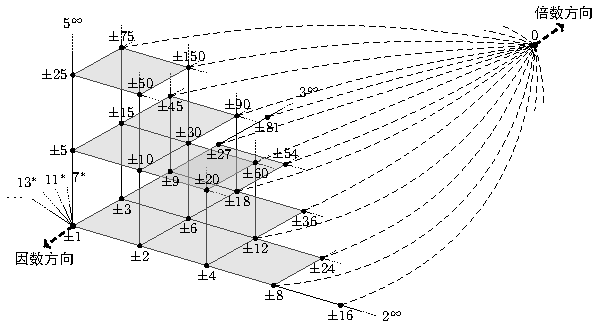
\includegraphics{pics/division_structure.pdf}
  \end{center}
\end{frame}

\begin{frame}
  \frametitle{标准分解式与 $p$ 进赋值序列}
  
  \begin{definition}
    对于正整数 $n$,设其标准分解式为 $n = p_1^{\alpha_1} p_2^{\alpha_2} \cdots p_k^{\alpha_k}$,对于给定素数 $p$,定义 $n$ 的 \fdf{$p$ 进阶数} $\nu_p(n) = \begin{cases} \alpha_i & \text{如果存在 $p_i = p$,} \\ 0 & \text{不存在 $p_i = p$。} \end{cases}$
    
    即,如果 $n$ 的 $p$ 进阶数 $\nu_p(n) = \alpha$,则 $p^\alpha \mid n$ 但 $p^{\alpha + 1} \nmid n$,此时也记作 $p^\alpha \parallel n$,如果 $p^\alpha \parallel n$ 不成立,记作 $p^\alpha \nparallel n$。
    
    \visible<2->{
      同时,定义 $n$ 的 \fdf{$p$ 进赋值序列}为 $\langle \nu_2(n), \nu_3(n), \nu_5(n), \ldots \rangle$。
    }
  \end{definition}
  
  \visible<3->{
    \begin{examples}[$p$ 进赋值序列]
      \begin{mymulticols}[l][l]{2}
        \raggedcolumns
        \begin{itemize}
          \item $1 \mapsto \langle 0, 0, 0, \ldots \rangle$
          \item $126 \mapsto \langle 1, 2, 0, 1, 0, \ldots \rangle$
        \end{itemize}
      \end{mymulticols}
    \end{examples}
  }
\end{frame}

\begin{frame}
  \frametitle{标准分解式与 $p$ 进赋值序列 -- 性质}
  
  由算术基本定理可知,每个正整数与其 $p$ 进赋值序列一一对应。
  
  \visible<2->{
    \emptyline
    
    反之,每个只有有限项非零的非负整数序列,在看作 $p$ 进赋值序列后,可以对应到所有正整数。
  }
  
  \visible<3->{
    \emptyline
    
    所以,可以使用 $p$ 进赋值序列来表示正整数,在 $p$ 进赋值序列的视角下,每个正整数均位于无穷维空间的一个整点上,而每个维度均对应一个素数。
    
    \begin{figure}
      \begin{tikzpicture}[remember picture, overlay]
        \node [xshift = .12\pdfpagewidth, yshift = -.26\pdfpageheight] at (current page.center) {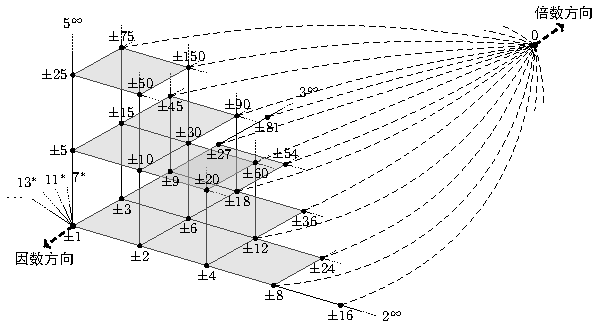
\includegraphics[scale = 0.6]{pics/division_structure.pdf}};
      \end{tikzpicture}
    \end{figure}
  }
\end{frame}

\begin{frame}
  \frametitle{标准分解式与 $p$ 进赋值序列 -- 结论}
  
  对于 $p$ 进阶数和 $p$ 进赋值序列,有如下结论:
  
  \begin{itemize}
    \item<2-> $\nu_p(a \cdot b) = \nu_p(a) + \nu_p(b)$。
    \item<2-> $a \mid b$ 等价于对于所有素数 $p$ 均有 $\nu_p(a) \le \nu_p(b)$。
    \item<2-> $\nu_p(\gcd(a, b)) = \min(\nu_p(a), \nu_p(b))$。
    \item<2-> $\nu_p(\lcm(a, b)) = \max(\nu_p(a), \nu_p(b))$。
    \item<3-> 于是,$\gcd(a, b) \cdot \lcm(a, b) = a \cdot b$ 是显然的。
  \end{itemize}
  
  \visible<4->{其中,$a, b$ 为非 $0$ 正整数,$p$ 为任意素数。}
  
  \visible<5->{
    \emptyline
    
    据此,可以证明 $a, b$ 的全体公因数就是 $\gcd(a, b)$ 的全体因数,\\
    \-\hspace{5em}以及 $a, b$ 的全体公倍数就是 $\lcm(a, b)$ 的全体倍数。
  }
\end{frame}

\begin{frame}
  \frametitle{标准分解式与 $p$ 进赋值序列 -- 完整图景}
  
  对于 $0$ 和负整数,可以如下定义它们的 $p$ 进阶数和 $p$ 进赋值序列:
  
  \begin{itemize}
    \item<2-> 对于任意素数 $p$,$0$ 的 $p$ 进阶数为 $\nu_p(0) = \infty$。\\
      $0$ 的 $p$ 进赋值序列为 $\langle \infty, \infty, \infty, \ldots \rangle$。
    \item<2-> 对于任意素数 $p$,负整数 $-n$ 的 $p$ 进阶数为 $\nu_p(-n) = \nu_p(n)$。\\
      $-n$ 的 $p$ 进赋值序列与 $n$ 的 $p$ 进赋值序列相同。
  \end{itemize}
  
  \visible<2->{
    如此,前述的 $\gcd$ 和 $\lcm$ 相关公式便可以拓展到 $0$ 和负整数。
  }
  
  \visible<3->{
    \emptyline
    
    并且,每个只有有限项非零的非负整数序列,在看作 $p$ 进赋值序列后,恰好对应一正一负两个整数。而序列 $\langle \infty, \infty, \infty, \ldots \rangle$ 对应在无穷维空间的无穷远点上的 $0$。
    
    于是,整除偏序在无穷维空间上的嵌入的结构便是清晰的了。
  }
\end{frame}

% \fi %%%%%%%%%%%%%%%%%%%%%%%%%%%%%%%%%%%%%%%%%%%%%%%%%%%%%%%%%%%

\section{基础算法}
\subsection{素性测试}
\subsubsection*{素性测试}

% \iffalse %%%%%%%%%%%%%%%%%%%%%%%%%%%%%%%%%%%%%%%%%%%%%%%%%%%%%%

\begin{frame}{素性测试}
  \fdf{素性测试},即判断一个正整数 $n$ 是否是素数。
  
  \visible<2->{
  \emptyline
    
    算法竞赛中,常用的素性测试算法有试除法和 Miller--Rabin 算法。Miller--Rabin 算法是一个多项式时间的素性测试算法,即它的最坏时间复杂度关于 $\log n$ 呈多项式增长。
  }
  
  \visible<3->{
    \emptyline
    
    一般的 Miller--Rabin 算法实现是非确定性的,有概率将合数报告为素数。对于确定性算法,有 Agrawal--Kayal--Saxena 算法同样是多项式时间的。
    
    \emptyline
    
    本课件中只介绍试除法。
  }
\end{frame}

\begin{frame}[fragile]
  \frametitle{试除法}
  
  \fdf{试除法}是素性测试的一种最简单的算法。
  
  \emptyline
  
  \pause
  
  试除法枚举所有在 $2$ 到 \only<3>{$n - 1$}\only<4>{\textboldcolor{orange}{$\left\lfloor \sqrt{n} \right\rfloor$}} 之间的整数 $d$,并通过计算 $n \bmod d$ 是否为 $0$ 判断 $d$ 是否为 $n$ 的因数。如果 $n \ne 1$ 并且不存在这样的因数,则可以确认 $n$ 是素数。%
  \pause%
  试除法的 \Cpp{} 代码:
  
  \begin{onlyenv}<3>
\begin{minted}[fontsize = \scriptsize]{cpp}
bool primality_test(int n) {
  for (int d = 2; d <= n - 1; ++d)
    if (n % d == 0)
      return false;
  return n != 1;
}
\end{minted}
  \end{onlyenv}
  
  \begin{onlyenv}<4>
\begin{minted}[fontsize = \scriptsize]{cpp}
bool primality_test(int n) {
  for (int d = 2; d * d <= n; ++d)
    if (n % d == 0)
      return false;
  return n != 1;
}
\end{minted}
  \end{onlyenv}
  
  可以看出,此算法的时间复杂度为 \only<3>{$\mathcal O (n)$}\only<4>{\textboldcolor{orange}{$\mathcal O \! \left( \sqrt{n} \right)$}}。
  
  \only<4>{此优化成立的原因是:如果 $n$ 拥有非平凡因数,则其最小非平凡正因数 $\le \sqrt{n}$。}
\end{frame}

% \fi %%%%%%%%%%%%%%%%%%%%%%%%%%%%%%%%%%%%%%%%%%%%%%%%%%%%%%%%%%%

\subsection{素因数分解}
\subsubsection*{素因数分解}

% \iffalse %%%%%%%%%%%%%%%%%%%%%%%%%%%%%%%%%%%%%%%%%%%%%%%%%%%%%%

\begin{frame}
  \frametitle{素因数分解}
  
  素因数分解,即给出一个正整数 $n$ 的标准分解式。
  
  \visible<2->{
    \emptyline
    
    算法竞赛中,常用的素因数分解算法有试除法和 Pollard's rho 算法。Pollard's rho 算法首先对 $n$ 执行任意素性测试算法,如果 $n$ 为合数,设 $n$ 的最小素因数为 $p$,该算法可以在 $\tilde{\mathcal O} \! \left( \sqrt{p} \right)$ 的时间复杂度内求出 $n$ 的一个非平凡因数 $a$。对 $a$ 和 $\frac{n}{a}$ 递归执行 Pollard's rho 算法即可完成素因数分解。
  }
  
  \visible<3->{
    \emptyline
    
    素因数分解在经典计算模型下是否有多项式时间算法还未知,目前最高效的算法为普通数域筛法。\\
    对于量子计算模型,有多项式时间的 Shor 算法。
    
    \emptyline
    
    本课件中只介绍试除法。
  }
\end{frame}

\begin{frame}{试除法}
  \fdf{试除法}是素因数分解的一种最简单的算法。
  
  \visible<2->{
    \emptyline
    
    与素性测试类似,素因数分解的试除法枚举所有 $2$ 到 $\left\lfloor \sqrt{n} \right\rfloor$ 之间的整数 $d$,并判断 $d$ 是否为 $n$ 的因数。\\
    如果 $d \mid n$,则 $d = p$ 必然为素数,然后不断从 $n$ 中除去素因数 $p$ 直到 $p \nmid n$,从 $n$ 中除去 $p$ 的次数即为 $\nu_p(n)$。\\
    注意,此时 $d$ 的枚举上限,即 $\left\lfloor \sqrt{n} \right\rfloor$,是会随着 $n$ 的减小而减小的,所以最终 $d$ 可能将不会枚举到原数的平方根处。\\
    最后,当由于 $d > \left\lfloor \sqrt{n} \right\rfloor$ 而退出循环后,如果 $n \ne 1$,则 $n$ 为原数的标准分解式中的最后一个素数。
  }
\end{frame}

\begin{frame}[fragile]{试除法 -- \Cpp{} 代码}
  试除法的 \Cpp{} 代码:
  
\begin{minted}[fontsize = \scriptsize]{cpp}
std::vector<std::pair<int, int>> prime_factorization(int n) {
  std::vector<std::pair<int, int>> ret;
  for (int d = 2; d * d <= n; ++d)
    if (n % d == 0) {
      int p = d, v = 0;
      while (n % p == 0)
        n /= p, ++v;
      ret.push_back({p, v});
    }
  if (n != 1)
    ret.push_back({n, 1});
  return ret;
}
\end{minted}
  
  可以看出,此算法的时间复杂度为 $\mathcal O \! \left( \sqrt{n} \right)$。
\end{frame}

% \fi %%%%%%%%%%%%%%%%%%%%%%%%%%%%%%%%%%%%%%%%%%%%%%%%%%%%%%%%%%%

\subsection{求最大公因数}
\subsubsection*{求最大公因数}

% \iffalse %%%%%%%%%%%%%%%%%%%%%%%%%%%%%%%%%%%%%%%%%%%%%%%%%%%%%%

\begin{frame}
  \frametitle{求最大公因数 -- Euclid 算法}
  
  求最大公因数,即给定两个非负整数 $a, b$,计算 $\gcd(a, b)$,是数论中一个很特别的问题,这是由于解决它的算法,即 \fdf{Euclid 算法},十分简单,而且有着非常优秀的时间复杂度。
  
  \emptyline
  
  注意,前文提到过,求非平凡因数在经典计算模型下是否有多项式时间算法还未知。事实上,包括 Pollard's rho 算法在内的许多数论算法都以 Euclid 算法为基础。
\end{frame}

\begin{frame}[fragile]{Euclid 算法}
  \only<1-2>{
    Euclid 算法基于如下结论:
    
    \begin{itemize}
      \item 当 $b = 0$ 时,$\gcd(a, b) = a$。
      \item 当 $b \ne 0$ 时,$\gcd(a, b) = \gcd(b, a \bmod b)$。
    \end{itemize}
    
    \visible<2->{
      \begin{proof}
        \renewcommand{\qedsymbol}{\visible<2->{(续)}}
        
        \begin{itemize}
          \item 当 $b = 0$ 时,由前文结论可知 $\gcd(a, b) = \gcd(a, 0) = a$。
        \end{itemize}
      \end{proof}
    }
  }
  
  \only<3>{
    \begin{itemize}
      \item 当 $b \ne 0$ 时,$\gcd(a, b) = \gcd(b, a \bmod b)$。
    \end{itemize}
    
    \begin{block}{证明(续).}
      \begin{itemize}
        \item 当 $b \ne 0$ 时,有关于整除的结论 $d \mid a \iff d \mid (a - k \cdot b)$,\\
          取 $k = \left\lfloor \frac{a}{b} \right\rfloor$ 即得 $d \mid a \iff d \mspace{5mu} \! \left| \mspace{5mu} \middle( a - \left\lfloor \frac{a}{b} \right\rfloor \cdot b \right)$。
          
          根据有余数的除法,有 $a - \left\lfloor \frac{a}{b} \right\rfloor \cdot b = a \bmod b$。
          
          于是 $(d \mid a) \land (d \mid b) \iff ( d \mid (a \bmod b)) \land (d \mid b)$。
          
          结合前文已证的 $(d \mid a) \land (d \mid b) \iff d \mid \gcd(a, b)$,可得 $d \mid \gcd(a, b) \iff d \mid \gcd(a \bmod b, b)$。
          
          由于 $\gcd(a, b)$ 和 $\gcd(a \bmod b, b)$ 都是正整数,得到最终结论 $\gcd(a, b) = \gcd(a \bmod b, b) = \gcd(b, a \bmod b)$。\hfill \qedsymbol
      \end{itemize}
    \end{block}
  }
\end{frame}

\begin{frame}[fragile]{Euclid 算法 -- \Cpp{} 代码实现}
  Euclid 算法基于如下结论
  
  \begin{itemize}
    \item 当 $b = 0$ 时,$\gcd(a, b) = a$。
    \item 当 $b \ne 0$ 时,$\gcd(a, b) = \gcd(b, a \bmod b)$。
  \end{itemize}
  
  \begin{visibleenv}<2->
    \emptyline
    
    直接利用如上结论,可以给出 Euclid 算法的 \Cpp{} 代码:
      
\begin{minted}{cpp}
int gcd_Euclidean(int a, int b) {
  return b ? gcd_Euclidean(b, a % b) : a;
}
\end{minted}
  \end{visibleenv}
  
  \visible<3->{
    \emptyline
    
    我们将证明 Euclid 算法的时间复杂度为 $\mathcal O \!\left( \log \frac{\min(a, b)}{\gcd(a, b)} \right)$。
    
    不过在此之前,我们先看 Euclid 算法的一个运行实例。
  }
\end{frame}

\begin{frame}{Euclid 算法 -- 例子}
  假设我们需要计算 $\gcd(46, 240)$,则 Euclid 算法经过如下递归得到结果:%
  %
  \begin{align*}
    \gcd(46, 240) &= \gcd(240, 46) & & \text{($46 \bmod 240 = 46$)} \\
    &= \gcd(46, 10) & & \text{($240 \bmod 46 = 10$)} \\
    &= \gcd(10, 6) & & \text{($46 \bmod 10 = 6$)} \\
    &= \gcd(6, 4) & & \text{($10 \bmod 6 = 4$)} \\
    &= \gcd(4, 2) & & \text{($6 \bmod 4 = 2$)} \\
    &= \gcd(2, 0) & & \text{($4 \bmod 2 = 0$)} \\
    &= 2 & & \text{($\gcd(a, 0) = a$)} \\
  \end{align*}
\end{frame}

\begin{frame}{Euclid 算法 -- 时间复杂度证明}
  称 Euclid 算法的一次递归为一步。
  
  \visible<2->{
    \emptyline
    
    如果给定的 $\langle a, b \rangle$ 有其中之一为 $0$,则算法将在 $2$ 步内结束。接下来假定 $a, b \ne 0$。
    
    如果 $a < b$,则算法的第 $1$ 步将交换 $a, b$,接下来假定 $a \ge b$。
  }
  
  \visible<3->{
    \emptyline
    
    有此结论:对于正整数 $a, b$,如果 $a \ge b$,则 $a \bmod b < \frac{a}{2}$。\\
    \-\hspace{2em}证明:如果 $b \le a < 2 \cdot b$,则 $a \bmod b = a - b < a - \frac{a}{2} = \frac{a}{2}$,\\
    \-\hspace{5em}否则 $a \ge 2 \cdot b$,则 $a \bmod b < b \le \frac{a}{2}$。
  }
  
  \visible<4>{
    \emptyline
    
    所以,在算法接下来的每一步,$a, b$ 两数中均有一个会变为原来的至多一半。总步数将被控制在 $\mathcal O (\log a + \log b)$ 内。
  }
\end{frame}

\begin{frame}{Euclid 算法 -- 时间复杂度证明(续)}
  又注意到,如果 $a \ge b$,则第 $1$ 步后两数为 $\langle b, a \bmod b \rangle$,两数均小于等于 $b$,接下来的时间复杂度为 $\mathcal O (\log b)$。所以,总步数将被控制在 $\mathcal O (\log \min(a, b))$ 内。
  
  \begin{visibleenv}<2>
    \emptyline
    
    又由于 Euclid 算法在计算 $\langle a, b \rangle$ 时的过程和 $\left\langle \frac{a}{\gcd(a, b)}, \frac{b}{\gcd(a, b)} \right\rangle$ 完全一致(后者在计算中的值乘 $\gcd(a, b)$ 即得到前者)。
    
    所以,Euclid 算法的时间复杂度为 $\mathcal O \!\left( \log \frac{\min(a, b)}{\gcd(a, b)} \right)$。
  \end{visibleenv}
\end{frame}

% \fi %%%%%%%%%%%%%%%%%%%%%%%%%%%%%%%%%%%%%%%%%%%%%%%%%%%%%%%%%%%

\section{素数筛法}

% \iffalse %%%%%%%%%%%%%%%%%%%%%%%%%%%%%%%%%%%%%%%%%%%%%%%%%%%%%%

\begin{frame}
  \frametitle{素数筛法 -- 引入}
  
  接下来我们关心的是与素数分布有关的问题:
  
  \begin{itemize}
    \item 如何求出第 $n$ 个素数?
    \item 如何求出小于等于 $n$ 的最大素数?
    \item 如何求出大于等于 $n$ 的最小素数?
    \item 在 $1 \sim n$ 的正整数中,一共有多少素数?
    \item ……
  \end{itemize}
  
  \visible<2>{
    \emptyline
    
    素数筛法可以解决这些问题,本课件中,我们介绍 Eratosthenes 筛法和 Euler 筛法。
  }
\end{frame}

% \fi %%%%%%%%%%%%%%%%%%%%%%%%%%%%%%%%%%%%%%%%%%%%%%%%%%%%%%%%%%%

\subsection{Eratosthenes 筛法}
\subsubsection*{Eratosthenes 筛法}

% \iffalse %%%%%%%%%%%%%%%%%%%%%%%%%%%%%%%%%%%%%%%%%%%%%%%%%%%%%%

\begin{frame}{小学五年级数学}
  \only<1>{让我们复习一下五年级下册数学(人教版)。}
  
  \only<2>{
    \begin{center}
      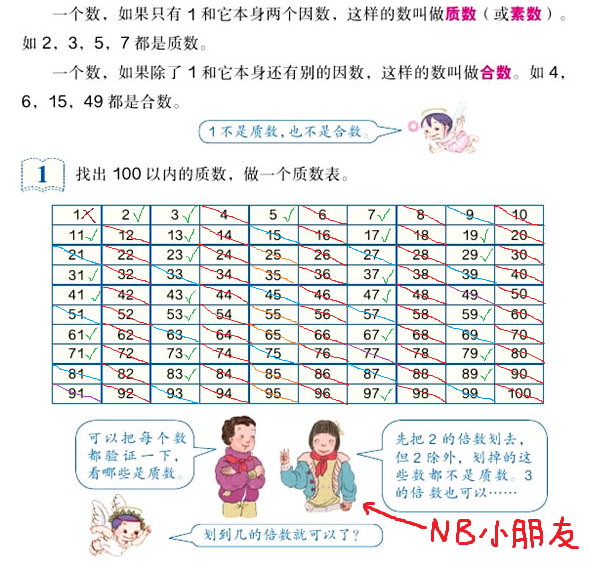
\includegraphics[scale = .38]{pics/prime.png}
    \end{center}
  }
\end{frame}

\begin{frame}{Eratosthenes 筛法}
  \only<1>{
    小明描述的算法相当于对 $1 \sim n$ 中每个数都进行一次素性测试。
    
    小红描述的过程就是 \fdf{Eratosthenes 筛法}。
    
    小天使的问题“划到几的倍数就可以了?”的回答是“划到 $\left\lfloor \sqrt{n} \right\rfloor$ 的倍数就可以了”。这与试除法中只对不超过 $\left\lfloor \sqrt{n} \right\rfloor$ 的数进行因数判断原因相同。
  }
  
  \only<2->{
    让我们再描述一次算法流程:
    
    \begin{enumerate}
      \item 维护一个下标范围在 $2 \sim n$ 的 Boolean 数组,表示每个数是否被划去,初始时所有数都未被划去。
      \item 从上一个找到的素数开始,找到数组中下一个未被划去的下标,将其标记为素数,并将其所有非本身的正倍数划去。
      \item 重复步骤 2,直到不存在下一个未被划去的下标或此下标大于 $\left\lfloor \sqrt{n} \right\rfloor$ 即可停止,这意味着 $2 \sim n$ 中的所有素数均已被找到。
      \item 将数组中剩余的未被划去的下标标记为素数。
    \end{enumerate}
    
    \emptyline
    
    算法结束后,所有的素数按照从小到大的顺序被找到,并且 Boolean 数组记录了每个数的素性:如果被划去则是合数,否则是素数。
  }
\end{frame}

\begin{frame}[fragile]{Eratosthenes 筛法 -- \Cpp{} 实现}
  以下是 Eratosthenes 筛法的 \Cpp{} 代码:
  
\begin{minted}[fontsize = \scriptsize]{cpp}
bool is_composite[MaxN];
std::vector<int> sieve_of_Eratosthenes(int n) {
  std::vector<int> primes;
  for (int i = 2; i <= n; ++i)
    if (!is_composite[i]) {
      primes.push_back(i);
      if ((long long)i * i <= n)
        for (int j = 2 * i; j <= n; j += i)
          is_composite[j] = true;
    }
  return primes;
}
\end{minted}
  
  \visible<2>{接下来将解释 Eratosthenes 筛法的时间复杂度为 $\mathcal O (n \log \log n)$。}
\end{frame}

\begin{frame}{Eratosthenes 筛法 -- 时间复杂度}
  Eratosthenes 筛法的时间复杂度由内层循环体的执行次数确定。即%
  \[%
    \text{复杂度} \sim \sum_{p \le \sqrt{n}} \left\lfloor \frac{n}{p} \right\rfloor \sim n \sum_{p \le \sqrt{n}} \frac{1}{p} \sim n \ln \ln \!\left( \sqrt{n} \right) = n \log \log n \text{。}
  \]%
  其中,基于一结论 $\displaystyle \sum_{p \le n} \frac{1}{p} = \ln \ln n + \mathcal O (1)$。\footnote{此结论即 Mertens 第二定理}
  
  \visible<2>{
    \emptyline
    
    运行在一般个人电脑上时,如前述朴素实现的 Eratosthenes 筛法可以在 1 秒内处理出 $2 \sim n = 3 \times {10}^7$ 甚至更大范围内的所有素数。
  }
\end{frame}

\begin{frame}{区间筛法}
  \begin{block}{问题 (区间求素数)}
    给定整数 $l, r$,求出 $l \sim r$ 内的所有素数。
    
    \begin{itemize}
      \item[\textbullet] 数据范围:$1 \le l \le r \le {10}^{14}$,$r - l \le {10}^7$。
    \end{itemize}
  \end{block}
  
  \visible<2->{
    可以对 Eratosthenes 筛法进行拓展以解决此问题。
    
    考虑使用 Eratosthenes 筛法求出 $1 \sim \left\lfloor \sqrt{r} \right\rfloor$ 内的所有素数。
    
    根据试除法中的结论,仅使用这些素数即可划去区间 $l \sim r$ 内的所有合数。与前文类似,时间复杂度可以分析为%
    %
    \begin{align*}
      & \phantom{{} = {}} \mathcal O \!\left( \sqrt{r} \log \log r \right) + \mathcal O ((r - l + 1) \log \log r) \\
      &= \mathcal O \!\left( \left( r - l + \sqrt{r} \right) \log \log r \right)\! \text{。}
    \end{align*}
  }
\end{frame}

% \fi %%%%%%%%%%%%%%%%%%%%%%%%%%%%%%%%%%%%%%%%%%%%%%%%%%%%%%%%%%%

\subsection{Euler 筛法}
\subsubsection*{Euler 筛法}

% \iffalse %%%%%%%%%%%%%%%%%%%%%%%%%%%%%%%%%%%%%%%%%%%%%%%%%%%%%%

\begin{frame}{对 Eratosthenes 筛法进行改造}
  注意到,在 Eratosthenes 筛法中,每个合数被其每个素因数均划去了一次。实际上,若使用 $\omega(n)$ 表示正整数 $n$ 的不同素因数个数,则 Eratosthenes 筛法的复杂度说明了 $\displaystyle \sum_{i = 1}^{n} \omega(i) = \mathcal O (n \log \log n)$。
  
  \visible<2->{
    \emptyline
    
    这启发我们改造 Eratosthenes 筛法,使得每个合数仅被其最小素因数划去。也即,每个素数 $p$ 不会划去最小素因数不为它的合数。
  }
  
  \visible<3->{
    \emptyline
    
    换句话说,考虑该合数为 $k = p \cdot i$,则 $i$ 应为一个最小素因数大于等于 $p$ 的正整数。\visible<4->{接下来,我们将展示改造后的算法的具体细节。}
  }
\end{frame}

\begin{frame}{Euler 筛法}
  Eratosthenes 筛法的此改造得名于 (Euler, 1737),即 \fdf{Euler 筛法}。
  
  \emptyline
  
  对于正整数 $n \ge 2$,记 $\lpd(n)$ 为 $n$ 的最小素因数。\\
  根据前文结果,在使用素数 $p$ 筛去其倍数 $k = p \cdot i$ 时,需要确保 $\lpd(i)$ 大于等于 $p$。\visible<2->{为了在对 $p$ 和 $i$ 的双重枚举中确保这一点,有以下两种实现手段:}
  
  \visible<2->{
    \begin{enumerate}
      \item 外层枚举素数 $p$,内层枚举乘数 $i$,内层需要确保 $\lpd(i) \ge p$。
      \item 外层枚举乘数 $i$,内层枚举素数 $p$,内层需要确保 $p \le \lpd(i)$。
    \end{enumerate}
  }
  
  \visible<3->{
    \emptyline
    
    在算法竞赛中,常见的是第 2 种实现手段。其原因是自然的:\\
    枚举 $p \le \lpd(i)$ 时,只需要从小到大枚举目前求出的素数 $p$,直到发现 $i \bmod p = 0$,即 $p \mid i$ 时跳出循环即可。
  }
\end{frame}

\begin{frame}[fragile]{Euler 筛法 -- \Cpp{} 实现}
  以下是 Euler 筛法的 \Cpp{} 代码:
  
\begin{minted}[fontsize = \scriptsize]{cpp}
bool is_composite[MaxN];
std::vector<int> sieve_of_Euler(int n) {
  std::vector<int> primes;
  for (int i = 2; i <= n; ++i) {
    if (!is_composite[i])
      primes.push_back(i);
    for (int p : primes) {
      int k = p * i;
      if (k > n) break;
      is_composite[k] = true;
      if (i % p == 0) break;
    }
  }
  return primes;
}
\end{minted}
\end{frame}

% \fi %%%%%%%%%%%%%%%%%%%%%%%%%%%%%%%%%%%%%%%%%%%%%%%%%%%%%%%%%%%

\section{解线性 Diophantus 方程}
\subsection{问题引入}
\subsubsection{线性 Diophantus 方程}

% \iffalse %%%%%%%%%%%%%%%%%%%%%%%%%%%%%%%%%%%%%%%%%%%%%%%%%%%%%%

\begin{frame}{Diophantus 方程}
  \begin{definition}
    \fdf{Diophantus 方程}指多元整系数方程,求解只在整数范围内进行。
  \end{definition}
  
  数论中的许多经典问题与 Diophantus 方程有关,我们通常关心特定形式的 Diophantus 方程是否有解,若有解则试图判断解数是否有限,若有无限组解则希望求出通解形式。
\end{frame}

\begin{frame}{Diophantus 方程 -- 例子}
  \begin{examples}[Diophantus 方程]
    \begin{itemize}
      \item<2-> 关于 $x, y, z$ 的方程 $x^n + y^n = z^n$ 为 Diophantus 方程。\\
        已知 $n = 1, 2$ 时,此方程的通解形式已得到清晰理解。\footnote<2->{Pythagorean 三元组}\\
        \-\hspace{2em} $n \ge 3$ 时,Fermat 猜想此方程仅有平凡解 $(0, 0, 0)$。\footnote<2->{Fermat 猜想 ($\sim$1637),Fermat 大定理 (Wiles, 1995)}
      \item<3-> 关于 
\includegraphics[align = c]{pics/fruits.pdf} 的方程 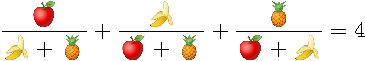
\includegraphics[align = c]{pics/fruits_equation.pdf} 通分后可以变为 Diophantus 方程的形式。\\
        据说有 $99 \%$ 的人无法找到正整数解。\footnote<3->{一组正整数解为}
    \end{itemize}
  \end{examples}
  
  \visible<3->{
    \begin{figure}
      \begin{tikzpicture}[remember picture,overlay]
        \node [xshift = .3775\pdfpagewidth, yshift = -.4945\pdfpageheight] at (current page.center) {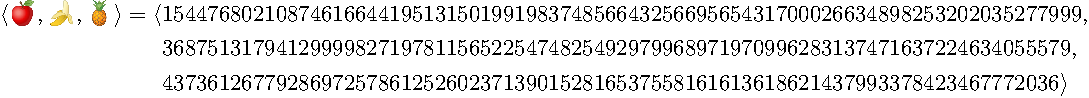
\includegraphics[scale = 0.82313]{pics/fruits_equation_solution.pdf}};
      \end{tikzpicture}
    \end{figure}
  }
\end{frame}

\begin{frame}{线性 Diophantus 方程}
  \begin{definition}
    关于 $x, y$ 的方程 $a x + b y = c$ 称为一个\fdf{线性 Diophantus 方程}。\\
    其中 $a, b, c$ 均为整数,并要求 $a, b$ 不能同时为 $0$。
  \end{definition}
  
  \visible<2->{
    \begin{examples}[线性 Diophantus 方程]
      \begin{itemize}
        \item $\phantom{1} x + \phantom{0}2 y = 0$ 为线性 Diophantus 方程。
        \item $6 x - 10 y = 4$ 为线性 Diophantus 方程。
        \item $6 x - 10 y = 3$ 为线性 Diophantus 方程。
        \item $0 x + \phantom{0}0 y = 0$ \alert{不}为线性 Diophantus 方程。
      \end{itemize}
    \end{examples}
  }
\end{frame}

\begin{frame}{线性 Diophantus 方程 -- 解集形式}
  \only<1>{
    \begin{examples}[线性 Diophantus 方程的解集]
      \begin{itemize}
        \item 线性 Diophantus 方程 $\phantom{1} x + \phantom{0}2 y = 0$ 的解集为\\
          \-\hspace{2em}$\langle x = -2 k, y = k \rangle$($k \in \mathbb Z$)。
        \item 线性 Diophantus 方程 $6 x - 10 y = 4$ 的解集为\\
          \-\hspace{2em}$\langle x = 4 + 5 k, y = 2 + 3 k \rangle$($k \in \mathbb Z$)。
        \item 线性 Diophantus 方程 $6 x - 10 y = 3$ 的解集为 $\varnothing$。
      \end{itemize}
    \end{examples}
  }
  
  \only<2>{
    可以看出,线性 Diophantus 方程的解集形式是以下二者之一:
    
    \begin{itemize}
      \item $\langle x_0 - k b', y_0 + k a' \rangle$($\langle x_0, y_0 \rangle$ 为一组特解,$k \in \mathbb Z$)
      \item $\varnothing$
    \end{itemize}
    
    \emptyline
    
    我们需要对某个特定方程的解集分类,并给出具体形式。
  }
\end{frame}

% \fi %%%%%%%%%%%%%%%%%%%%%%%%%%%%%%%%%%%%%%%%%%%%%%%%%%%%%%%%%%%

\subsubsection{线性同余方程与有理数取模}

% \iffalse %%%%%%%%%%%%%%%%%%%%%%%%%%%%%%%%%%%%%%%%%%%%%%%%%%%%%%

\begin{frame}{线性同余方程}
  \begin{definition}
    \fdf{线性同余方程}指关于 $x$ 的形如 $a x \equiv b \pmod{m}$ 的同余方程。\\
    其中 $m$ 为正整数,$a, b$ 为整数。
  \end{definition}
  
  \begin{visibleenv}<2->
    \begin{examples}[线性同余方程]
      \begin{itemize}
        \item $\phantom{1}x \equiv 0 \pmod{\phantom{0}2}$ 为线性同余方程。
        \item $6 x \equiv 4 \pmod{10}$ 为线性同余方程。
        \item $6 x \equiv 3 \pmod{10}$ 为线性同余方程。
      \end{itemize}
    \end{examples}
  \end{visibleenv}
\end{frame}

\begin{frame}{线性同余方程 -- 解集形式}
  \begin{examples}[线性同余方程的解集]
    \begin{itemize}
      \item 线性同余方程 $\phantom{1}x \equiv 0 \pmod{\phantom{0}2}$ 的形式已足够简洁,解集为\\
        \-\hspace{2em}$x \equiv 0 \pmod{2}$。
      \item 线性同余方程 $6 x \equiv 4 \pmod{10}$ 的解集为\\
        \-\hspace{2em}$x \equiv 4 \pmod{5}$。
      \item 线性同余方程 $6 x \equiv 3 \pmod{10}$ 的解集为 $\varnothing$。
    \end{itemize}
  \end{examples}
  
  \begin{visibleenv}<2->
    可以看出,线性同余方程的解集形式是以下二者之一:
    
    \begin{mymulticols}[l][l]{2}
      \begin{itemize}
        \item $x \equiv x_0 \pmod{m'}$
        \item $\varnothing$
      \end{itemize}
    \end{mymulticols}

    \emptyline
    
    我们需要对某个特定方程的解集分类,并给出具体形式。
  \end{visibleenv}
\end{frame}

\begin{frame}{线性同余方程 -- 与线性 Diophantus 方程的联系}
  事实上,有线性同余方程 $a x \equiv b \pmod{m}$ 与 $m \mid (a x - b)$ 等价,并进一步等价于存在 $k$ 使得 $k m = a x - b$ 成立,令 $y = -k$,移项后变为 $a x + m y = b$,可以看作一个关于 $x, y$ 的线性 Diophantus 方程。
  
  \begin{visibleenv}<2->
    \emptyline
    
    这意味着,只需要解决 $a x + m y = b$ 这一线性 Diophantus 方程,即可解决原线性同余方程。
  \end{visibleenv}
\end{frame}

\begin{frame}{有理数取模}
  \begin{onlyenv}<1>
    目前我们已经定义整数对另一正整数的模,也即进行有余数的除法后得到的余数。
    
    \emptyline
    
    从同余等价的角度考虑,对于有理数来说,我们也希望通过同余关系定义有理数对一正整数的模,并期望如此定义的模保持运算性质。
  \end{onlyenv}
  
  \begin{onlyenv}<2-3>
    \begin{definition}[有理数取模]
      给定正整数 $m$,定义 $({\ast} \mathbin{\mathrm{mod}_{\mathbb Q}} m) : \mathbb Q \to \{ 0, 1, \ldots, m - 1 \}$,保持:
      
      \begin{itemize}
        \item 对于整数 $n$,$n \mathbin{\mathrm{mod}_{\mathbb Q}} m = n \bmod m$
        \item $((a \mathbin{\mathrm{mod}_{\mathbb Q}} m) \pm (b \mathbin{\mathrm{mod}_{\mathbb Q}} m)) \bmod m = (a \pm b) \mathbin{\mathrm{mod}_{\mathbb Q}} m$
        \item $((a \mathbin{\mathrm{mod}_{\mathbb Q}} m) \cdot (b \mathbin{\mathrm{mod}_{\mathbb Q}} m)) \bmod m = (a \cdot b) \mathbin{\mathrm{mod}_{\mathbb Q}} m$
      \end{itemize}
      
      其中,$a, b$ 为任意有理数。
    \end{definition}
    
    \begin{visibleenv}<3->
      然而,注意到,当我们取 $a = m$ 而 $b = \frac{1}{m}$ 时,如果 $b \mapsto x$,则必须有 $0 \cdot x \equiv 1 \pmod{m}$,而这当 $m \ne 1$ 时是不可能的。
    \end{visibleenv}
  \end{onlyenv}
\end{frame}

\begin{frame}{有理数取模 -- 困难与联系}
  正如前文所述,在定义 $m \ne 1$ 时的有理数取模时遇到了困难。
  
  \begin{visibleenv}<2->
    \emptyline
    
    让我们考虑一有理数的最简分数表示为 $x = \frac{b}{a}$,则根据上述定义,需要满足 $((a \mathbin{\mathrm{mod}_{\mathbb Q}} m) \cdot (x \mathbin{\mathrm{mod}_{\mathbb Q}} m)) \bmod m = b \mathbin{\mathrm{mod}_{\mathbb Q}} m$。
  \end{visibleenv}
  
  \begin{visibleenv}<3->
    令 $x' = x \mathbin{\mathrm{mod}_{\mathbb Q}} m$。上式即%
    %
    \[ a x' \equiv b \pmod{m} \text{。} \]
    %
    即一线性同余方程。如果此方程有解,则有希望定义有理数 $x$ 对 $m$ 的模。
  \end{visibleenv}
  
  \begin{visibleenv}<4->
    \emptyline
    
    而线性同余方程可以被转化为线性 Diophantus 方程。接下来我们将展示线性 Diophantus 方程的求解方法。
  \end{visibleenv}
\end{frame}

% \fi %%%%%%%%%%%%%%%%%%%%%%%%%%%%%%%%%%%%%%%%%%%%%%%%%%%%%%%%%%%

\subsection{问题解决}
\subsubsection{Bézout 定理}

% \iffalse %%%%%%%%%%%%%%%%%%%%%%%%%%%%%%%%%%%%%%%%%%%%%%%%%%%%%%

\begin{frame}{Bézout 定理}
  为了解决方程 $a x + b y = c$,首先考察当 $x, y$ 任取时,$a x + b y$ 的取值。接下来我们给出 \fdf{Bézout 定理(Bézout's lemma)}。
  
  \begin{visibleenv}<2-3>
    \begin{theorem}[Bézout 定理]
      回顾前文提到过的 $a_1, a_2, \ldots, a_n$ 的整系数线性组合。\\
      令 $g = \gcd(a_1, a_2, \ldots, a_n)$,则 $a_{1 \sim n}$ 的所有整系数线性组合恰好就是 $g$ 的所有倍数。
    \end{theorem}
  \end{visibleenv}
  
  \begin{visibleenv}<3>
    \begin{examples}[Bézout 定理]
      \begin{itemize}
        \item 当 $a = [ 6, 12, 16 ]$ 时,$a$ 的整系数线性组合有 $\{ \ldots, -4, -2, 0, 2, 4, \ldots \}$,其中 $2 = \gcd(6, 12, 16)$。
      \end{itemize}
    \end{examples}
  \end{visibleenv}
\end{frame}

\begin{frame}{Bézout 定理 -- 证明}
  \begin{onlyenv}<1-7>
    \begin{proof}[Bézout 定理]
      \renewcommand{\qedsymbol}{\visible<7>{\leavevmode (续)}}
      
      \visible<2->{当 $g = 0$,即 $a_{1 \sim n}$ 均为 $0$ 时,定理显然成立。接下来假定 $g \ge 1$。}
      
      \visible<3->{
        \emptyline
        
        若 $g \ge 1$ 则说明至少有一个 $a_k \ne 0$,则 $a$ 的整系数线性组合中至少有一正元素 $|a_k|$。取 $s$ 为 $a$ 的整系数线性组合中的\alert{最小正元素}。
      }
      
      \visible<4->{考虑进行有余数的除法,令 $a_i$ 除以 $s$ 的商为 $q$,余数为 $r$。那么有 $r = a_i - q \cdot s$,同样是一个整系数线性组合。}
      
      \visible<5->{然而 $0 \le r < s$,结合 $s$ 的最小性,只能有 $r = 0$,这说明 $s \mid a_i$。}
      
      \visible<6->{由 $i$ 的任意性,这说明 $s$ 是 $a_{1 \sim n}$ 的一个公因数。于是 $s \mid g$。}
      
      \visible<7>{然而 $g$ 应整除任意整系数线性组合,即 $g \mid s$。于是只能有 $g = s$。}
    \end{proof}
  \end{onlyenv}
  
  \begin{onlyenv}<8-10>
    \begin{proof}[Bézout 定理(续)]
      \renewcommand{\qedsymbol}{\visible<10>{\leavevmode \hbox {\usebeamertemplate *{qed symbol}}}}
      
      \visible<8->{已证 $g$ 即为所有整系数线性组合中的最小正元素。}
      
      \visible<9->{若某一整系数线性组合 $x$ 不是 $g$ 的倍数,则根据已证结论,$\gcd(g, x)$ 也为一整系数线性组合。然而由于 $g \nmid x$,有 $0 < \gcd(g, x) < g$,与 $g$ 的最小性矛盾。}
      
      \visible<10>{故所有整系数线性组合均是 $g = \gcd(a_1, a_2, \ldots, a_n)$ 的倍数。又有整系数线性组合的倍数自然也为整系数线性组合,故所有整系数线性组合恰好就是 $g = \gcd(a_1, a_2, \ldots, a_n)$ 的所有倍数。}
    \end{proof}
  \end{onlyenv}
\end{frame}

\begin{frame}{解的存在性判定}
  Bézout 定理解决了线性 Diophantus 方程的解的存在性判定问题。
  
  对于 $a x + b y = c$,令 $g = \gcd(a, b)$,则方程有解等价于 $g \mid c$。
  
  \begin{visibleenv}<2->
    \emptyline
    
    方程有解时,对于解的结构,Bézout 定理并未给出更多信息。
  \end{visibleenv}
\end{frame}

% \fi %%%%%%%%%%%%%%%%%%%%%%%%%%%%%%%%%%%%%%%%%%%%%%%%%%%%%%%%%%%

\subsubsection{齐次情况}

% \iffalse %%%%%%%%%%%%%%%%%%%%%%%%%%%%%%%%%%%%%%%%%%%%%%%%%%%%%%

\begin{frame}{齐次情况}
  考察当 $c = 0$ 时的齐次情况:$a x + b y = 0$。
  
  \begin{onlyenv}<2-4>
    若在所有整数上枚举 $y$ 的取值,对 $x$ 解得 $x = -\frac{b y}{a}$。
    
    要让 $x$ 为整数,需要 $a \mid b y$。
    
    \begin{visibleenv}<3->
      \emptyline
      
      从 $p$ 进赋值序列的视角考虑,即%
      %
      \begin{align*}
        \nu_p(a) & \le \nu_p(b) + \nu_p(y)\text{,} \\
        \text{这等价于\ } \nu_p(y) & \ge \max(\nu_p(a) - \nu_p(b), 0) \\
        & = \nu_p(a) - \min(\nu_p(b), \nu_p(a)) \\
        & = \nu_p \!\left( \tfrac{a}{\gcd(a, b)} \right)\! \text{。}
      \end{align*}%
    \end{visibleenv}%
    %
    \begin{visibleenv}<4->
      即 $y$ 应为 $\frac{a}{\gcd(a, b)}$ 的倍数。
    \end{visibleenv}
  \end{onlyenv}
  
  \begin{onlyenv}<5->
    设 $y = k \cdot \frac{a}{\gcd(a, b)}$,解得 $x = -k \cdot \frac{b}{\gcd(a, b)}$,代回原式验证:%
    %
    \[
      a \cdot \!\left( -k \cdot \frac{b}{\gcd(a, b)} \right)\! + b \cdot \!\left( k \cdot \frac{a}{\gcd(a, b)} \right) = 0
    \]%
    %
    确实成立。
    
    \emptyline
    
    \begin{visibleenv}<6->
      也即,令 $a' = \frac{a}{\gcd(a, b)}$ 和 $b' = \frac{b}{\gcd(a, b)}$,\\
      \-\hspace{3em}有通解形式 $\langle x, y \rangle = \langle -k b', k a' \rangle$。
    \end{visibleenv}
  \end{onlyenv}
\end{frame}

\begin{frame}{齐次情况 -- 特解与通解}
  如上给出了齐次情况的通解形式 $\langle -k b', k a' \rangle$,这大大简化了问题。
  
  \begin{visibleenv}<2->
    \emptyline
    
    这是因为,考虑 $a x + b y = c$ 的一特解 $\langle x_0, y_0 \rangle$,则此特解加上任意齐次情况下的解 $\langle x_1, y_1 \rangle$ 得到的 $\langle x_0 + x_1, y_0 + y_1 \rangle$ 必然也是原方程的解。
    
    反之,任意原方程的解 $\langle x_2, y_2 \rangle$ 都能通过与特解 $\langle x_0, y_0 \rangle$ 相减得到齐次情况下的解 $\langle x_0 - x_2, y_0 - y_2 \rangle$。
  \end{visibleenv}
  
  \begin{visibleenv}<3->
    \emptyline
    
    也即,$a x + b y = c$ 的解集必然呈现一特解 $\langle x_0, y_0 \rangle$ 加上任意齐次情况下的通解 $\left\langle -k \cdot \frac{b}{\gcd(a, b)}, k \cdot \frac{a}{\gcd(a, b)} \right\rangle$ 的形式。
  \end{visibleenv}
  
  \begin{visibleenv}<4->
    \emptyline
    
    接下来只需解决求出一组特解的问题即可。
  \end{visibleenv}
\end{frame}

% \fi %%%%%%%%%%%%%%%%%%%%%%%%%%%%%%%%%%%%%%%%%%%%%%%%%%%%%%%%%%%

\subsubsection{扩展 Euclid 算法}

% \iffalse %%%%%%%%%%%%%%%%%%%%%%%%%%%%%%%%%%%%%%%%%%%%%%%%%%%%%%

\begin{frame}{扩展 Euclid 算法 -- 引入}
  Bézout 定理显示了 $a x + b y = \gcd(a, b)$ 必定有解。\\
  进一步地,注意到 $a x + b y = c$ 有解当且仅当 $\gcd(a, b) \mid c$,则求出 $a x + b y = \gcd(a, b)$ 的一组特解 $\langle x_0, y_0 \rangle$ 后,将其乘 $\frac{c}{\gcd(a, b)}$ 后即可得到 $a x + b y = c$ 的一组特解。
  
  \begin{visibleenv}<2->
    \emptyline
    
    接下来介绍\fdf{扩展 Euclid 算法}以解决 $a x + b y = \gcd(a, b)$ 的特解问题。注意到 Bézout 定理给出的形式中带有 $\gcd(a, b)$,这启发我们改造 Euclid 算法,这也就是算法的名字由来。
  \end{visibleenv}
\end{frame}

\begin{frame}{扩展 Euclid 算法}
  \begin{onlyenv}<1-2>
    Euclid 算法依赖有余数的除法进行,其递归形式形如:%
    %
    \[
      \SetTblrInner{colsep = 0pt}
      \begin{tblr}{r @{{}={}} l @{{}\cdot{}} l @{{}+{}} l}
        a & q_1 & b & r_1 \\
        b & q_2 & r_1 & r_2 \\
        r_1 & q_3 & r_2 & r_3 \\
        \SetCell[c = 4]{c} \vdots & & & \\
        r_{n - 2} & q_n & r_{n - 1} & r_n \\
        r_{n - 1} & q_{n + 1} & r_n & r_{n + 1}
      \end{tblr}
    \]%
    %
    其中 $r_{n + 1} = 0$,于是递归过程在计算 $\gcd(r_n, r_{n + 1})$ 时停止。
    
    最终有 $g = \gcd(a, b) = r_n$。
    
    \begin{visibleenv}<2>
      \emptyline
      
      当计算 $\gcd(r_n, r_{n + 1})$ 时有 $1 \cdot r_n + 0 \cdot r_{n + 1} = g$,此即为边界。
    \end{visibleenv}
  \end{onlyenv}
  
  \begin{onlyenv}<3-4>
    考察连续两层递归 $\gcd(r_{i - 2}, r_{i - 1}) \rightleftharpoons \gcd(r_{i - 1}, r_i)$,它基于:%
    %
    \[
      r_{i - 2} = q_i \cdot r_{i - 1} + r_i \text{。}
    \]%
    %
    假设已求出 $x_{i + 1} \cdot r_{i - 1} + y_{i + 1} \cdot r_i = g$。
    
    现在要求 $x_i \cdot r_{i - 2} + y_i \cdot r_{i - 1} = g$ 的一组特解。
    
    \begin{visibleenv}<4>
      考虑 $r_i = {\color{red}r_{i - 2}} {\color{blue}{}- q_i} \cdot {\color{magenta}r_{i - 1}}$,将其代入 ${\color{cyan}x_{i + 1}} \cdot {\color{magenta}r_{i - 1}} + {\color{orange}y_{i + 1}} \cdot r_i = g$ 得%
      %
      \begin{align*}
        {\color{cyan}x_{i + 1}} \cdot {\color{magenta}r_{i - 1}} + {\color{orange}y_{i + 1}} \cdot ({\color{red}r_{i - 2}} {\color{blue}{}- q_i} \cdot {\color{magenta}r_{i - 1}}) &= g \\
        \implies {\color{orange}y_{i + 1}} \cdot {\color{red}r_{i - 2}} + ({\color{cyan}x_{i + 1}} {\color{blue}{}- q_i} \cdot {\color{orange}y_{i + 1}}) \cdot {\color{magenta}r_{i - 1}} &= g \text{。}
      \end{align*}%
      %
      于是有 $\langle x_i, y_i \rangle = \langle {\color{orange}y_{i + 1}}, {\color{cyan}x_{i + 1}} {\color{blue}{}- q_i} \cdot {\color{orange}y_{i + 1}} \rangle$。根据此式从边界 $\langle x_{n + 2}, y_{n + 2} \rangle = \langle 1, 0 \rangle$ 一步步回溯至 $\langle x_1, y_1 \rangle$ 即得原方程的一组特解。
    \end{visibleenv}
  \end{onlyenv}
\end{frame}

\begin{frame}[fragile]{扩展 Euclid 算法 -- \Cpp{} 实现}
  以下是扩展 Euclid 算法的 \Cpp{} 代码(\Cpp{}17):
  
\begin{minted}[fontsize = \scriptsize]{cpp}
std::pair<int, int> extended_Euclidean(int a, int b) {
  if (!b) return {1, 0};
  const auto &[x, y] = extended_Euclidean(b, a % b);
  return {y, x - a / b * y};
}
\end{minted}
  
  \begin{visibleenv}<2->
    在 \Cpp{}98 标准下可过编译的代码:
    
\begin{minted}[fontsize = \scriptsize]{cpp}
int extended_Euclidean(int a, int b, int &x, int &y) {
  if (!b) return x = 1, y = 0, a;
  int d = extended_Euclidean(b, a % b, y, x);
  return y -= a / b * x, d;
}
\end{minted}
  \end{visibleenv}
  
  \begin{visibleenv}<3->
    扩展 Euclid 算法的递归过程与 Euclid 算法相同,于是其时间复杂度也为 $\mathcal O \!\left( \log \frac{\min(a, b)}{\gcd(a, b)} \right)$。
  \end{visibleenv}
\end{frame}

\begin{frame}[c]{扩展 Euclid 算法 -- 例子}
  \[
    \SetTblrInner{colsep = 0pt}
    \begin{tblr}{colspec = {crcrcrcrcrcrrcrcrcrcc}, column{5, 12} = {rightsep+ = 7pt}, column{6, 13} = {leftsep+ = 7pt}, vline{6, 13}}
      \gcd({} & 240 & {},{} & 46 & {}) & \SetCell[c = 7]{c} & & & & & & & {\color{cyan}-9} & {}\cdot{} & {\color{magenta}240} & {\color{orange}{}+{}} & {\color{orange}47} & {}\cdot{} & 46 & {}={} & 2 \\
      \SetCell[c = 5]{c} \downarrow & & & & & {\color{red}240} & {}={} & {\color{blue}5} & {}\cdot{} & {\color{magenta}46} & {}+{} & 10 & \SetCell[c = 9]{c} \uparrow & & & & & & & & \\
      \gcd({} &  46 & {},{} & 10 & {}) & \SetCell[c = 7]{c} & & & & & & & {\color{cyan} 2} & {}\cdot{} & {\color{magenta} 46} & {\color{orange}{}-{}} & {\color{orange} 9} & {}\cdot{} & 10 & {}={} & 2 \\
      \SetCell[c = 5]{c} \downarrow & & & & & {\color{red} 46} & {}={} & {\color{blue}4} & {}\cdot{} & {\color{magenta}10} & {}+{} &  6 & \SetCell[c = 9]{c} \uparrow & & & & & & & & \\
      \gcd({} &  10 & {},{} &  6 & {}) & \SetCell[c = 7]{c} & & & & & & & {\color{cyan}-1} & {}\cdot{} & {\color{magenta} 10} & {\color{orange}{}+{}} & {\color{orange} 2} & {}\cdot{} &  6 & {}={} & 2 \\
      \SetCell[c = 5]{c} \downarrow & & & & & {\color{red} 10} & {}={} & {\color{blue}1} & {}\cdot{} & {\color{magenta} 6} & {}+{} &  4 & \SetCell[c = 9]{c} \uparrow & & & & & & & & \\
      \gcd({} &   6 & {},{} &  4 & {}) & \SetCell[c = 7]{c} & & & & & & & {\color{cyan} 1} & {}\cdot{} & {\color{magenta}  6} & {\color{orange}{}-{}} & {\color{orange} 1} & {}\cdot{} &  4 & {}={} & 2 \\
      \SetCell[c = 5]{c} \downarrow & & & & & {\color{red}  6} & {}={} & {\color{blue}1} & {}\cdot{} & {\color{magenta} 4} & {}+{} &  2 & \SetCell[c = 9]{c} \uparrow & & & & & & & & \\
      \gcd({} &   4 & {},{} &  2 & {}) & \SetCell[c = 7]{c} & & & & & & & {\color{cyan} 0} & {}\cdot{} & {\color{magenta}  4} & {\color{orange}{}+{}} & {\color{orange} 1} & {}\cdot{} &  2 & {}={} & 2 \\
      \SetCell[c = 5]{c} \downarrow & & & & & {\color{red}  4} & {}={} & {\color{blue}2} & {}\cdot{} & {\color{magenta} 2} & {}+{} &  0 & \SetCell[c = 9]{c} \uparrow & & & & & & & & \\
      \gcd({} &   2 & {},{} &  0 & {}) & \SetCell[c = 7]{c} & & & & & & & {\color{cyan} 1} & {}\cdot{} & {\color{magenta}  2} & {\color{orange}{}+{}} & {\color{orange} 0} & {}\cdot{} &  0 & {}={} & 2 \\
    \end{tblr}
  \]
\end{frame}

\begin{frame}{扩展 Euclid 算法 -- 特解的最小性}
  当对不能同时为 $0$ 的非负整数 $a, b$ 运行如上编写的扩展 Euclid 算法时,有性质:
  
  \begin{itemize}
    \item<2-> 如果 $b \mid a$\ \hspace{1em}\ $\phantom{a \mid b}$,那么将解得 $0 \cdot a + 1 \cdot b = \gcd(a, b) = b$。
    \item<2-> 如果 $b \nmid a$ 且 $a \mid b$,那么将解得 $1 \cdot a + 0 \cdot b = \gcd(a, b) = a$。
    \item<3-> 如果 $b \nmid a$ 且 $a \nmid b$,那么将解得的 $\langle x, y \rangle$ 满足%
      %
      \begin{center}
        $|x| \le \frac{b}{2 \gcd(a, b)}$ 以及 $|y| \le \frac{a}{2 \gcd(a, b)}$。
      \end{center}
  \end{itemize}
  
  \begin{visibleenv}<4>
    这意味着解得的 $\langle x, y \rangle$ 是所有解中绝对值最小的一组,并且同时说明算法运行过程中无需担心整型溢出的问题,将 $x, y$ 使用与 $a, b$ 相同的类型存储就足够了。
  \end{visibleenv}
\end{frame}

\begin{frame}{解线性 Diophantus 方程 -- 总结}
  解线性 Diophantus 方程 $a x + b y = c$ 时只需进行下列步骤。
  
  \begin{enumerate}
    \item<2-> 用扩展 Euclid 算法求 $a x + b y = \gcd(a, b)$ 的特解 $\langle x_0, y_0 \rangle$。
    \item<3-> 判断是否有 $\gcd(a, b) \mid c$,如果 $\gcd(a, b) \nmid c$ 则无解。
    \item<4> 如果 $\gcd(a, b) \mid c$,则原方程通解形式为($k \in \mathbb Z$):%
      %
      \[
        \left\{ \begin{aligned}
          x = c' \cdot x_0 - k \cdot b' \\
          y = c' \cdot y_0 + k \cdot a'
        \end{aligned} \right.
      \]%
      %
      其中 $a' = \frac{a}{\gcd(a, b)}$ 且 $b' = \frac{b}{\gcd(a, b)}$ 且 $c' = \frac{c}{\gcd(a, b)}$。
  \end{enumerate}
\end{frame}

\begin{frame}{线性同余方程 -- 伏笔回收}
  如前文所述,线性同余方程 $a x \equiv b \pmod{m}$ 可转化为线性 Diophantus 方程 $a x + m y = b$ 的求解。
  
  \emptyline
  
  若 $a x + m y = b$ 通解为 $\langle x_0 + k m', y_0 + k a' \rangle$($k \in \mathbb Z$),\\
  则 $a x \equiv b \pmod{m}$ 的解有形式 $x \equiv x_0 \pmod{m'}$。
  
  其中 $m' = \frac{m}{\gcd(a, m)}$。
  
  \emptyline
  
  若 $a x + m y = b$ 无解,即 $\gcd(a, m) \nmid b$,则 $a x \equiv b \pmod{m}$ 也无解。
  
  只有当 $\gcd(a, m) \ne 1$ 时才有可能发生无解的情况(回顾线性 Diophantus 方程的解的存在性判定条件)。
\end{frame}

\begin{frame}{有理数取模 -- 伏笔回收}
  如前文所述,为最简分数 $\frac{b}{a}$ 定义对 $m$ 的模时,可以考虑线性同余方程 $a x \equiv b \pmod{m}$ 的解。
  
  \emptyline
  
  假设 $a x \equiv b \pmod{m}$ 有解 $x \equiv x_0 \pmod{m'}$,其中 $m' = \frac{m}{\gcd(a, m)}$。
  
  \begin{itemize}
    \item 如果 $m' = m$,即 $\gcd(a, m) = 1$,也即 $a \perp m$,\\
      \-\hspace{2em}可以定义 $\frac{b}{a} \mathbin{\mathrm{mod}_{\mathbb Q}} m = x_0 \bmod m$。
    \item 如果 $m' \ne m$,即 $\gcd(a, m) \ne 1$,这是不可能的,因为有解当且仅当 $\gcd(a, m) \mid b$,于是这说明 $\gcd(a, b) \ne 1$,故 $\frac{b}{a}$ 并非最简分数,与前提矛盾。
  \end{itemize}
  
  \emptyline
  
  得出结论:最简分数 $\frac{b}{a}$ 的模有定义当且仅当 $a \perp m$。
\end{frame}

\begin{frame}{有理数取模 -- 乘法逆元}
  如前文所述,最简分数 $\frac{b}{a}$ 的模有定义当且仅当 $a \perp m$。
  
  考虑模的性质:$(a \mathbin{\mathrm{mod}_{\mathbb Q}} m) \cdot (b \mathbin{\mathrm{mod}_{\mathbb Q}} m) \equiv (a \cdot b) \mathbin{\mathrm{mod}_{\mathbb Q}} m$。
  
  于是有 $\frac{b}{a}$ 的模等于 $b$ 的模乘 $\frac{1}{a}$ 的模。
  
  故只需要定义全体与 $m$ 互质的正整数 $a$ 的倒数 $\frac{1}{a}$ 的模即可。
  
  假设 $\frac{1}{a}$ 的模为 $x$,则 $x$ 将会满足 $a x \equiv 1 \pmod{m}$,在同余式的运算中扮演消去一侧 $a$ 因子的角色:%
  %
  \begin{align*}
    (\mathcal A) \cdot a &\equiv \mathcal B \\
    (\mathcal A) \cdot a \cdot x &\equiv (\mathcal B) \cdot x \\
    \mathcal A &\equiv (\mathcal B) \cdot x
  \end{align*}%
  %
  我们称满足 $a x \equiv 1 \pmod{m}$ 的 $x$ 为 $a$ 模 $m$ 的\fdf{乘法逆元}。
  
  可以证明模 $m$ 同余的所有 $a$ 的乘法逆元相同,并且扩展 Euclid 算法给出了乘法逆元的一种计算方法。
\end{frame}

\begin{frame}[c]
  \centering
  \begin{beamercolorbox}[sep = 12pt, center]{section title}
    \usebeamerfont{section title}感谢倾听\par
  \end{beamercolorbox}
\end{frame}

% \fi %%%%%%%%%%%%%%%%%%%%%%%%%%%%%%%%%%%%%%%%%%%%%%%%%%%%%%%%%%%

\section{附录}
\subsection*{附录}

\begin{frame}[c]{中英文对照表}
  \tiny
  
  \begin{adjustwidth}{-.5cm}{}
    \begin{mymulticols}[l][l]{3}
      \begin{itemize}
        \item 整除:divide
        \item 被……整除:be divided by
        \item 倍数:multiple
        \item 因数(约数):divisor,factor
        \item 平凡因数(平凡约数):trivial divisor,trivial factor
        \item 整系数线性组合:linear combination with integer coefficients
        \item 商:quotient
        \item 余数:remainder
        \item 素数(质数):prime number
        \item 合数:composite number
        \item 同余:congruent
        \item 模:modulo
        \item 模数:modulus
        \item 公因数(公约数):common divisor,common factor
        \item 最大公因数(最大公约数):greatest common divisor,highest common factor
        \item 互素(互质):coprime,relatively prime,mutually prime
        \item 公倍数:common multiple
        \item 最小公倍数:least common multiple,smallest common multiple
        \item 算术基本定理(唯一分解定理):fundamental theorem of arithmetic,unique factorization theorem
        \item 标准分解式:canonical representation,standard form
        \item $p$ 进阶数:$p$-adic order
        \item $p$ 进赋值:$p$-adic valuation
        \item 素性测试:primality test
        \item 试除法:trial division
        \item 素因数分解(分解素因数、质因数分解、素因子分解):prime factorization
        \item Euclid(欧几里得)算法:Euclidean algorithm
        \item Eratosthenes(埃拉托斯特尼)筛法:sieve of Eratosthenes
        \item Euler(欧拉)筛法:Euler's sieve,sieve of Euler
        \item Diophantus(丢番图)方程:Diophantine equation
        \item 线性同余方程:linear congruence equation
        \item Bézout(裴蜀)定理:Bézout's lemma
        \item 扩展 Euclid(欧几里得)算法:extended Euclidean algorithm
        \item 乘法逆元:modular multiplicative inverse
      \end{itemize}
    \end{mymulticols}
  \end{adjustwidth}
\end{frame}

\begin{frame}[c]{参考文献与致谢}
  \begin{itemize}
    \item OI Wiki,\url{https://oi-wiki.org/}
    \item Wikipedia,\url{https://en.wikipedia.org/}
    \item 具体数学(\textit{Concrete Mathematics: A Foundation for Computer Science}),R.~L.~Graham, D.~E.~Knuth, and O.~Patashnik
    \item 数论导引,华罗庚
    \item 本课件编写时的哔哩哔哩直播间观众
  \end{itemize}
\end{frame}

\end{document}